% 
% Annual Cognitive Science Conference
% Sample LaTeX Paper -- Proceedings Format
% 

% Original : Ashwin Ram (ashwin@cc.gatech.edu)       04/01/1994
% Modified : Johanna Moore (jmoore@cs.pitt.edu)      03/17/1995
% Modified : David Noelle (noelle@ucsd.edu)          03/15/1996
% Modified : Pat Langley (langley@cs.stanford.edu)   01/26/1997
% Latex2e corrections by Ramin Charles Nakisa        01/28/1997 
% Modified : Tina Eliassi-Rad (eliassi@cs.wisc.edu)  01/31/1998
% Modified : Trisha Yannuzzi (trisha@ircs.upenn.edu) 12/28/1999 (in process)
% Modified : Mary Ellen Foster (M.E.Foster@ed.ac.uk) 12/11/2000
% Modified : Ken Forbus                              01/23/2004
% Modified : Eli M. Silk (esilk@pitt.edu)            05/24/2005
% Modified : Niels Taatgen (taatgen@cmu.edu)         10/24/2006
% Modified : David Noelle (dnoelle@ucmerced.edu)     11/19/2014

%% Change "letterpaper" in the following line to "a4paper" if you must.

\documentclass[10pt,letterpaper]{article}

\usepackage{cogsci}
\usepackage{pslatex}
\usepackage{apacite}

\usepackage{graphicx}

\title{Using Pupillometry as a Surrogate for Brain Reward Feedback with Commodity Hardware and Software}
% \title{How to Make a Proceedings Paper Submission}

\author{{\large \bf Martin Diges (mdiges@wisc.edu)} \\
    Department of Computer Science, 1210 W. Dayton Street \\
    Madison, WI 53706 USA
    }
% \author{{\large \bf Morton Ann Gernsbacher (MAG@Macc.Wisc.Edu)} \\
%   Department of Psychology, 1202 W. Johnson Street \\
%   Madison, WI 53706 USA
%   \AND {\large \bf Sharon J.~Derry (SDJ@Macc.Wisc.Edu)} \\
%   Department of Educational Psychology, 1025 W. Johnson Street \\
%   Madison, WI 53706 USA}


\begin{document}

\maketitle


\begin{abstract}
Prior work suggests that measurements of pupil diameter, pupillometry, can reveal some information about an individual's inner mental state, a prominent example of which being information about recent rewards. Can measures of pupil diameter captured using commodity hardware and software be used as proxies for reward feedback as it is perceived in the brain? 
% The abstract should be one paragraph, indented 1/8~inch on both sides,
% in 9~point font with single spacing. The heading ``{\bf Abstract}''
% should be 10~point, bold, centered, with one line of space below
% it. This one-paragraph abstract section is required only for standard
% six page proceedings papers.

\textbf{Keywords:} 
pupillometry; reward signaling; commodity hardware
% \textbf{Keywords:} 
% add your choice of indexing terms or keywords; kindly use a
% semicolon; between each term
\end{abstract}

\section{Background and Motivation}
% Start by motivating your research question,
A Brain Computer Interface (BCI), is a type of human-machine interface that reads signals from the brain, typically electric signals, and translates them into desired actions. These devices are developed in a clinical setting most often for persons with significantly reduced motor control and can allow those persons to control a wheelchair, use a computer, or plainly just communicate.

A BCI must be learn to interpret a user's brain signals in order to help them perform tasks appropriately. One way to teach a BCI is through Supervised Learning (SL), where the user is exposed to stimuli (which can include proprioceptive stimulus) that elicit brain signals associated with their intent to perform a task. The BCI makes a prediction and compares its prediction to what the user's "true intent" is. Suminski et al. (2010) demonstrate an instance of this Supervised Learning in the context of training a BCI to move a robot arm on behalf of a nonhuman primate. SL requires a "ground truth" against which the BCI may compare their prediction, hence a dataset is needed of "true" robot arm movements. This approach poses an important issue, which is that such "ground truth" data may not be readily available. This hampers the autonomy that BCIs are meant to provide, as the persons using them may require controlled training for each new task they wish their BCI to perform. 

Reinforcement Learning is another approach to training BCIs. Rather than compare its prediction to a "true intent", the BCI receives feedback on how good its prediction is through some other mean. The advantage with using RL is that the BCI only needs a reward signal as opposed to ground truth data. If a person has the ability to specify the reward correspondent to the BCI's predictions, the BCI can improve at their task over time without the need for a special dataset, a controlled training environment, or a visit to a facility.

The final issue that remains is that individuals with heavily reduced motor function may have trouble providing this feedback to the BCI.

In their review of reinforcement learning BCI approaches, Girdler, Caldbeck, and Bae (2022) highlight existing work, including An et al. (2019), which provide evidence for obtaining such a reward signal directly from a person's brain. Thus, the thought goes, if reward can be obtained from the person's brain, they need only be able to assess the BCI's performance at a mental level in order for the BCI to learn.

Predicting reward from brain signals works for BCIs with access to the inside of the skull, but what if one would like to obtain a reward signal without having to place electrodes on/inside the skull? Pupillometry, the analysis of pupil diameter dynamics, is one such approach. Work by Kloosterman et al. (2015) suggests that changes in pupil size at constant light levels may be reflective of some brain state, and in particular that pupil dynamics can encode some of the surprise and content of perceptual events.

\begin{figure*}[h]
    \centering
    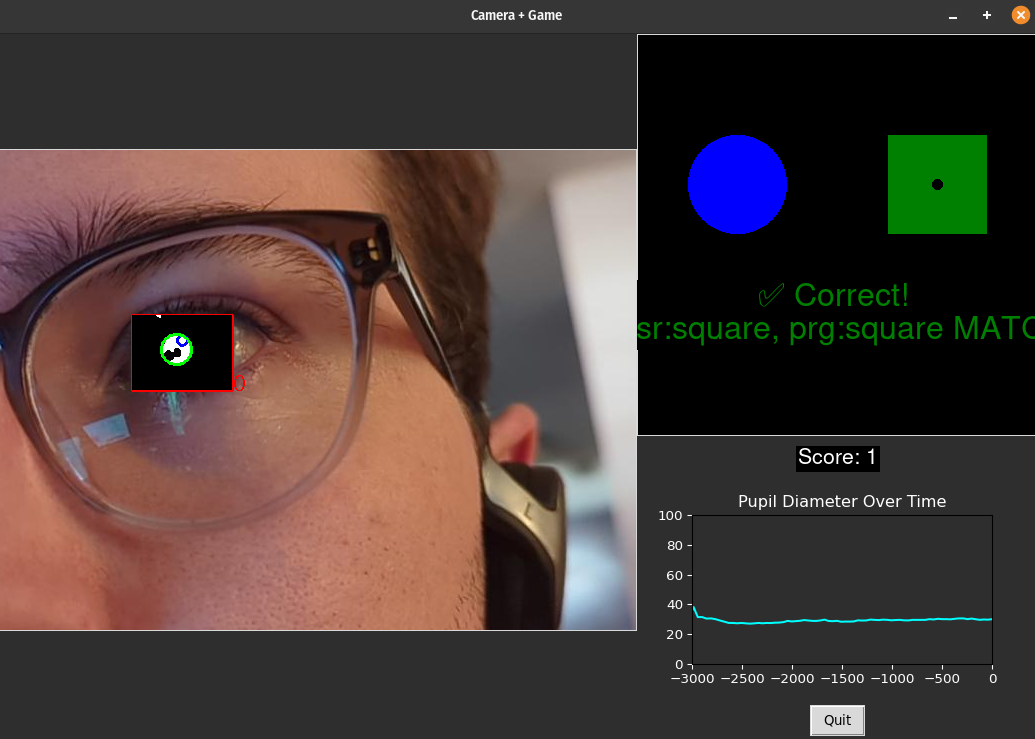
\includegraphics[width=0.7\linewidth]{course_project/figures/screenshot_GUI.png}
    \caption{Screenshot from the GUI program during operation}
    \label{fig:enter-label}
\end{figure*}

\section{Question}
% succinctly state your question
If pupil diameter can carry some information about events being perceived, could pupillometry be used as a surrogate for brain reward feedback?

% and
% outline the structure of the paper

% \section{Background}\
% Next, provide the background for your project, providing context to
% your question and discussing any previous work on it.



\section{Method}
% Then, describe your methods

\begin{figure*}[h]
    \centering
    \includegraphics[width=1\linewidth]{course_project/figures/figure_traces_2025-05-06 20:16:44.png}
    \caption{Preprocessing carried out ahead of analysis. Vertical dashed line indicates the time at which reward was administered to the user.
    \textbf{(a)} Pupil diameter samples from the time interval 500ms before to 1000ms after reward is given. Each trace corresponds to the diameter samples from a single trial. Horizontal dashed lines are placed 4 L1 norm distances from the all-trial mean pupil diameter. Traces which exceed this threshold are marked for removal.
    \textbf{(b)} Same information as (a), only with the outlier traces removed.
    \textbf{(c)} Same traces as shown in (b), with the horizontal dashed lines removed and traces now colored according to whether the shape chosen was correct or not.
    }
    \label{fig:enter-label}
\end{figure*}

A microphone stand was modified and set up such that it could hold a camera and so that it could be moved close to a participant's face when desired. To provide a live video feed, a Google Pixel 8 phone was placed on the stand, connected to a computer via a stock USB-C cable (with data transfer capabilities), and it was made to act as a webcam through its USB settings. This provided a significantly superior image quality compared to a regular webcam, which doesn't fare well when close to one's face.

On the same computer, a simple GUI program was created in Python 3.13 using the built-in "tkinter" GUI library. A screenshot of this GUI program is shown in Figure 1. The GUI displays the camera feed to the user. The program uses OpenCV code to detect eyes in the camera feed's frames. Further code locates the likely pupil within the eye area. The predicted pupil diameter is overlaid on the camera feed for the user's convenience. The GUI also plots pupil diameter over time as diameter readings come in.

\subsection{Task}
Finally, the GUI displays a simple 2-alternative forced choice (2AFC) game for the user to play. Two shapes are present side by side. During a single trial, the player may choose between the two shapes by pressing the arrow keys on their keyboard. One of the shapes is the "correct" shape and will inform the player of their correct choice visually and with a pleasant auditory queue. The other shape provides corresponding visual feedback on the player's incorrect choice and also provides a less pleasant auditory queue. The visual feedback is kept small so as to try to avoid pupil dynamics caused by changes in screen luminosity. As the player chooses correctly, the "correct" shape may change with some probability after a successful trial.

The user's pupil diameter is recorded for the duration of the GUI being open and is written to disk. When analysis begins, the pupil trajectories for each of the trials are aggregated within a range of time around the time of the user being rewarded. This range is (-500, +1000) ms so as to capture some of the steady-state pupil diameter before reward is provided and how the pupil diameter evolves after the reward is provided. Figure 2 shows the preprocessing that these traces undergo. Firstly, the L1 norm of the pupil diameter across all trials is calculated. Trials wherein the pupil diameter goes further from the mean than 4 times this norm are considered outliers and are marked for removal. Outliers can pop up as a result of the imperfect pupil diameter detection system used, as it can momentarily lose track of the pupil. Secondly, the trials are coded according to whether the reward administered was positive or negative. Lastly, as is seen in Figure 3 in the results section, pupil diameter samples are binned into 50ms segments of time so that samples can be aggregated over trials.

%%% RESULTS
\section{Results}

\begin{figure*}[h]
    \centering
    \includegraphics[width=1\linewidth]{course_project/figures/figure_means_2025-05-06 20:16:44.png}
    \caption{After outlier trials are removed and remaining trials are labeled according to choice correctness, 
    \textbf{(d)} samples have their timestamps binned into 50ms buckets.
    \textbf{(e)} The mean trajectory is computed for Correct and Incorrect trials. 95\% Confidence intervals are shown.
    \textbf{(f)} Owing to the high trial-specific bias in pupil diameter, each trial has its pre-reward mean pupil diameter computed and subtracted from all trial samples.
    \textbf{(g)} Once per-trial means are removed, mean trajectories are once again computed for Correct and Incorrect trials. 95\% Confidence intervals are shown.
    }
    \label{fig:enter-label}
\end{figure*}
% and results
Figure 3 shows our main results. Once the pupil diameter samples are binned (d), they have their mean plotted with a 95\% non-parametric CI (e). There does not appear to be a statistically significant difference between pupil diameter before the reward time.

From (d), it was observed that there was some per-trial bias in the pupil diameter. This is a consequence of the imperfect camera setup where the participant's head was not stationary and hence small head movements could periodically change the steady state pupil diameter. Hence in (f) each trial has its pre-reward mean pupil diameter computed and subtracted from all trial samples. What we see are traces that have much of their per-trial bias removed. Finally, in (g) we take the mean of these "de-meaned" (not literally, of course) trajectories and again plot it with a 95\% CI. The confidence intervals once again indicate no statistically significant difference before the reward time. Though not statistically significant at a confidence of 95\%, the plot in (g) suggests that there may be a difference between the post-reward pupil diameter of correct/incorrect trials that could be used to predict reward.

%%% DISCUSSION
\section{Discussion}
The type of reward signal being examined during this experiment is not what would be used to train a BCI. A BCI would require feedback on its predictions, whereas the task presented to the player in this paper does not have a model making predictions from user input and thus does not elicit such feedback. The type of reward feedback examined in this paper could most closely be described as the player's perception of their own performance. The machinery to elicit the prior type of feedback was present in the code but went unused primarily owing to how confusing it made the task and the limitation on statistical power described below. Further work would address these two concerns.

The number of trials used after filtering was quite small (n=142), hence my hypothesis is that with a greater number of trials there may be a statistically significant difference in pupil diameter between correct and incorrect trials. This limitation was present due to the inconsistency in steady-state pupil diameter between recording sessions, itself a consequence of the physical setup of the experiment not keeping the subject's head a steady distance from the camera. The consequence of this session-to-session difference in steady-state pupil diameter is that samples cannot readily be aggregated across sessions, hence only samples from a single session could be reliably used. 142 is just about the most trials that could be tolerated while staying still with eyes wide open. It should be possible to address this limitation, but constraints on time leave this for future development.


%%% Conclusion
\section{Conclusion}
In this paper we discussed an attempt at differentiating brain reward state through pupil dynamics observed by commodity hardware and software.

While the difference in pupil dynamics was not significant at a 95\% level, the overall shape of the intervals does motivate the aggregation of more sessions to see whether a statistically significant difference can be found.

% \section{General Formatting Instructions}

% The entire contribution of a proceedings paper (including figures,
% references, and anything else) can be no longer than six pages.

% The text of the paper should be formatted in two columns with an
% overall width of 7 inches (17.8 cm) and length of 9.25 inches (23.5
% cm), with 0.25 inches between the columns. Leave two line spaces
% between the last author listed and the text of the paper. The left
% margin should be 0.75 inches and the top margin should be 1 inch.
% \textbf{The right and bottom margins will depend on whether you use
%   U.S. letter or A4 paper, so you must be sure to measure the width of
%   the printed text.} Use 10~point Times Roman with 12~point vertical
% spacing, unless otherwise specified.

% The title should be in 14~point, bold, and centered. The title should
% be formatted with initial caps (the first letter of content words
% capitalized and the rest lower case). Each author's name should appear
% on a separate line, 11~point bold, and centered, with the author's
% email address in parentheses. Under each author's name list the
% author's affiliation and postal address in ordinary 10~point type.

% Indent the first line of each paragraph by 1/8~inch (except for the
% first paragraph of a new section). Do not add extra vertical space
% between paragraphs.


% \section{First Level Headings}

% First level headings should be in 12~point, initial caps, bold and
% centered. Leave one line space above the heading and 1/4~line space
% below the heading.


% \subsection{Second Level Headings}

% Second level headings should be 11~point, initial caps, bold, and
% flush left. Leave one line space above the heading and 1/4~line
% space below the heading.


% \subsubsection{Third Level Headings}

% Third level headings should be 10~point, initial caps, bold, and flush
% left. Leave one line space above the heading, but no space after the
% heading.


% \section{Formalities, Footnotes, and Floats}

% Use standard APA citation format. Citations within the text should
% include the author's last name and year. If the authors' names are
% included in the sentence, place only the year in parentheses, as in
% \citeA{NewellSimon1972a}, but otherwise place the entire reference in
% parentheses with the authors and year separated by a comma
% \cite{NewellSimon1972a}. List multiple references alphabetically and
% separate them by semicolons
% \cite{ChalnickBillman1988a,NewellSimon1972a}. Use the
% ``et~al.'' construction only after listing all the authors to a
% publication in an earlier reference and for citations with four or
% more authors.


% \subsection{Footnotes}

% Indicate footnotes with a number\footnote{Sample of the first
% footnote.} in the text. Place the footnotes in 9~point type at the
% bottom of the column on which they appear. Precede the footnote block
% with a horizontal rule.\footnote{Sample of the second footnote.}

% \subsection{Tables}

% Number tables consecutively. Place the table number and title (in
% 10~point) above the table with one line space above the caption and
% one line space below it, as in Table~\ref{sample-table}. You may float
% tables to the top or bottom of a column, or set wide tables across
% both columns.

% \begin{table}[!ht]
% \begin{center} 
% \caption{Sample table title.} 
% \label{sample-table} 
% \vskip 0.12in
% \begin{tabular}{ll} 
% \hline
% Error type    &  Example \\
% \hline
% Take smaller        &   63 - 44 = 21 \\
% Always borrow~~~~   &   96 - 42 = 34 \\
% 0 - N = N           &   70 - 47 = 37 \\
% 0 - N = 0           &   70 - 47 = 30 \\
% \hline
% \end{tabular} 
% \end{center} 
% \end{table}

% \subsection{Figures}

% All artwork must be very dark for purposes of reproduction and should
% not be hand drawn. Number figures sequentially, placing the figure
% number and caption, in 10~point, after the figure with one line space
% above the caption and one line space below it, as in
% Figure~\ref{sample-figure}. If necessary, leave extra white space at
% the bottom of the page to avoid splitting the figure and figure
% caption. You may float figures to the top or bottom of a column, or
% set wide figures across both columns.

% \begin{figure}[ht]
% \begin{center}
% \fbox{CoGNiTiVe ScIeNcE}
% \end{center}
% \caption{This is a figure.} 
% \label{sample-figure}
% \end{figure}

\section{Acknowledgments}

This paper was inspired by preliminary findings made while working with faculty and researchers from the University of Wisconsin - Madison's Department of Neuroscience. Thank you to Aaron Suminski, Luis Populin, and Abigail Rajala for their mentorship.

This paper was created for Comp Sci / Psych 841, taught by Joseph Austerweil. Thank you to Joe Austerweil for being an encouraging instructor and for making sure I kept my expectations realistic. Without their feedback I likely would not have finished this work in time.

% \section{References Instructions}

% Follow the APA Publication Manual for citation format, both within the
% text and in the reference list, with the following exceptions: (a) do
% not cite the page numbers of any book, including chapters in edited
% volumes; (b) use the same format for unpublished references as for
% published ones. Alphabetize references by the surnames of the authors,
% with single author entries preceding multiple author entries. Order
% references by the same authors by the year of publication, with the
% earliest first.

% Use a first level section heading, ``{\bf References}'', as shown
% below. Use a hanging indent style, with the first line of the
% reference flush against the left margin and subsequent lines indented
% by 1/8~inch. Below are example references for a conference paper, book
% chapter, journal article, dissertation, book, technical report, and
% edited volume, respectively.

\nocite{AnENEURO.0178-19.2019}
\nocite{Suminski2010}
\nocite{Kloosterman2015}
\nocite{Girdler2022}

\bibliographystyle{apacite}

\setlength{\bibleftmargin}{.125in}
\setlength{\bibindent}{-\bibleftmargin}

\bibliography{course_project/Diges_2025}

\end{document}

% \nocite{ChalnickBillman1988a}
% \nocite{Feigenbaum1963a}
% \nocite{Hill1983a}
% \nocite{OhlssonLangley1985a}
% % \nocite{Lewis1978a}
% \nocite{Matlock2001}
% \nocite{NewellSimon1972a}
% \nocite{ShragerLangley1990a}